\documentclass[free]{flammie}

 \usepackage{microtype}
 \usepackage{graphicx}
 \usepackage{linguex}
\usepackage{tikz-dependency}
\usepackage{multicol}
\usepackage{xurl}


\title{How to Create Treebanks without Human Annotators---An Indigenous
Language Grammar Checker for Treebank
Construction\footnotepubrights{\aclanthologypostprintdoi{2025.tlt-1.14}}
    }

\author{Linda Wiechetek \\
   \\
   \\
  \texttt{first.last@uit.no} \\\and%
  Flammie A Pirinen  \\
  UiT---Norgga árktalaš universitehta \\
  Tromsø, Norway \\
  \texttt{first.last@uit.no} \\\and%
  Maja Lisa Kappfjell \\
   \\
   \\
  \texttt{first.last@uit.no}
  }

\begin{document}

\maketitle
\begin{abstract}
   Creating treebanks for low resource languages is an important task.  However,
    low resource Indigenous language contexts have not only limited resources in
    terms of text data, but also limited human resources that are available for
    linguistic annotation.  We suggest a work-around by applying a Constraint
    Grammar operated rule-based dependency parser to do the work of creating a
    marked-up treebank. However, due to a lot of noise, meaning spelling and
    grammatical errors in South Sámi written texts, this tool often fails to
    create complete and correct trees.  As a fix to this, we created a grammar
    checking tool for the most common South Sámi grammatical error types, which
    improves the quality of the dependency parser significantly.  As both
    literacy and normative standards for most Indigenous languages are much more
    recent than for majority languages, spelling and grammatical variation and
    errors are a common source of noise, and the application of a correction
    tool like ours can be useful in the construction of treebanks for these
    languages.
\end{abstract}


\section{Introduction}

In an extremely low resource language context, treebanks are an important link
to developing high level tools that other languages consider standard.

Machine-learning based language technology can utilise the treebanks for
training and testing new models, and rule-based systems can use them as a gold
standard to strive for.  In addition they can be used for language comparative
tasks, evaluation, etc.  Low resource languages like South Sámi, however, are
not only low resource in terms of data ($<$ 2 million words) but also lack human
resources, which makes manual linguistic annotation of big text corpora
impossible.  For creating a South Sámi treebank, we therefore applied a
Constraint Grammar based dependency annotation tool that can annotate unlimited
amounts of text automatically using existing morphological and syntactic tools
as their basis.  When dealing with low resource Indigenous languages we need to
keep in mind that language standards are often still in the process of being
developed, and language contact with the majority language influences the way
people use their language. South Sámi texts contain a lot of noise in each
sentence in terms of typos and non-standard forms, code-switching and sentence
structures that resemble literal translations from the majority language rather
than using authentic South Sámi syntax.  This type of noise is not comparable to
the noise in a majority language corpus. It rather reflects the relatively large
amount of L2 writers (second language users) in the South Sámi text corpus. As
we want a treebank that can also be used for teaching purposes, we would like it
to represent mostly L1 language.

Some of these errors and non-standard forms disrupt the sentential dependency
structures and prevent our tool from working properly. Especially noun phrase
internal errors, case errors and agreement errors lead to broken dependency
trees.  We therefore suggest the usage of a spelling and \textit{grammar error
correction} (GEC) tool as part of the pipeline to create a treebank. All our
tools are part of a multi-lingual language resource platform (\textit{GiellaLT})
which provides a common infrastructure for over 150 languages, most of them
low-resource and/or Indigenous
languages.\footnote{\url{https://giellalt.github.io} and
\url{https://giellalt.github.io/LanguageModels.html}} We manually marked-up
error corpora, which we used to identify relevant and frequent errors and
created a grammar checking tool that corrects these morpho-syntactic structures.
The corrected sentences are then fed into the dependency tool, which create our
treebank for South Sámi.

South Sámi is an Indigenous language with about 500 speakers, and about 10
percent of these writes the language.

This work has been made within a language technology group that started as an
initiative of the Sámi Parliament 20 years ago, which is why we combine both
native language and engineering competence. Our main goal is to develop tools
for and together with the language community, especially those that are needed
in administration and education. This is self-determination in practice, which
is also central principle in Sámi endeavors.

South Sámi is a Uralic language with interesting syntactic features, such as
copula drop, which leaves many sentences without a finite verb, an interesting
matter for dependency parsing.

This work is a contribution to creating both proofing tools and a treebank for
further research and tool creation.  South Sámi did not previously have an
annotated treebank, thus our contribution in this work is also that of a new
treebank.  Our goal was to create in the most efficient way given limited
resources, also making sure that language presented therein is authentic but
error free.  The treebank follows the written standard that is backed by the
South Sámi standardization body \textit{Gïelegaaltije} creating a valuable
annotated corpus resource.

We will in the following present the grammar checking tool, and show how it is
integrated into automatic treebank construction of South Sámi.

\section{Background}

\subsection{Language background}

South Sámi is an official language in altogether four municipalities in Norway
and six municipalities in Sweden. There are approximately 300--600 South Sámi
speakers. South Sámi is a morphologically complex language with similar
grammatical structures as other Sámi languages. The Sámi languages belong to the
Uralic language family, which is unrelated to the Indo-European languages. South
Sámi has a number of features that clearly distinguish it from other Sámi
languages. South Sámi has even stronger SOV word order than Lule Sámi, and both
distinguish between elative and inessive case, which are replaced by locative
case in North Sámi. South Sámi typically drops the copula in sentences without
pro-drop. It also has nominative plural noun phrases in definite object
position, which influences syntactic disambiguation. Negation is more complex
than in North and Lule Sámi as South Sámi has a specific paradigm for past tense
copula negation verbs that agree with the negation forms.  The South Sámi
written standard or according to the term of the time, The South Sámi textbook
standard, was recommended by the Sámi Language Council in 1976 and was adopted
in 1978.~\cite{Bergsland1993} Some grammatical variants and paradigms have not
yet been standardized explicitly by the standardization organ
(\textit{Gïelegaaltije}). However, there are written grammars that serve as a
basis for teaching and for proofreading. A few grammatical matters are not
described in grammars yet, and the grammatical authority lays with the native
speaker elders.  This knowledge remains to be formalized and presented in a way
such that newer speakers that are less exposed to the language can receive the
guiding they need to be confident speakers and writers.

Language contact with the Scandinavian majority languages Norwegian and Swedish
are further leading to a lot of interference in South Sámi written text. These
are clearly marked because they deviate significantly from both Sámi and Uralic
morpho-syntax.  A clear South Sámi standard is essential for the survival of the
language. Without a clear standard new learners lack the confidence to use the
language in speech and script and typically chose the safer alternative, the
majority language.  This means that language planning requires clear choices as
regard orthography, lexicon, idioms and grammar to ensure a future for South
Sámi and discontinue the colonialization process.

\subsection{Technical background}

The core pieces of this work are a rule-based dependency analyzer and a grammar
checker module.  The dependency analyzer is written for the three Sámi
languages, North Sámi, Lule Sámi and South Sámi, which is based on a full
morphological analysis that is followed by morpho-syntactic disambiguation and
syntactic parsing. The syntactic parsing includes only function labels, but no
explicit dependencies. Until this step the different Sámi languages have their
separate language modules. The dependency structure, however, is added in a
common module for all the languages, based on the flat syntactic function tags
from the previous module. This work is thoroughly described
in~\cite{antonsen-etal-2010-reusing}.  The automatic dependency annotation is
created bottom up, so that even partial dependency trees can be created if some
parts of the sentence contain errors or could not be fully disambiguated.
Dependencies build on the same syntactic structure as the grammar checker.  They
use a specific rule format, which maps dependents to their parents and the other
way around based on previously mapped morpho-syntactic labels and word order.
The parsing of dependencies is based on rules of the type shown in
Figure~\ref{fig:dependency}, for example where we map the object to a transitive
main verb to its right.


\begin{figure}
{\texttt{%
SETPARENT:SetObjToRightMv OBJ> TO (*1 (<mv>) BARRIER S-BOUNDARY OR @-FSUBJ>);
}}
    \caption{Example rule mapping objects to their right handed verbal
    mothers\label{fig:dependency}}
\end{figure}

\begin{figure}
    \centering
    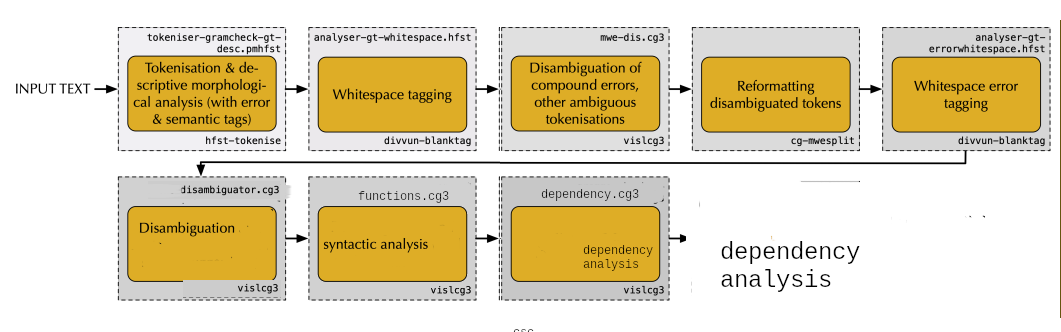
\includegraphics[width=.5\textwidth ]{syntaxflow.png}
    \caption{Modular structure of the dependency
    analysis\label{fig:dependencyflow}}
\end{figure}

The grammar checker module uses the same technology and a similar pipeline. It
is specifically written for South Sámi, although some of the error types exist
in North and Lule Sámi as well.

Our framework is based on rule-based natural language processing: finite-state
morphology~\cite{beesley2003finite} and constraint
grammar~\cite{karlsson1990constraint}.  We use the free/ open source VISL CG 3
\textit{constraint grammar} (CG) compiler~\cite{bick2015cg}.  The linguistic
analyses made by the systems include morphological, syntactic and semantic
analyses, both on word-level as well as on a dependency graph level.  The VISL
CG 3 -based dependency analysis has been used in various applications including
grammar checking, machine translation, semantic role annotation for various
languages like Greenlandic, Danish, Spanish,
Portuguese.~\cite{bick2019dependency,rademaker2017universal,bick2022modular}

The VISL CG 3 dependency analysis' foremost goal is not to build a treebank with
complete trees, but primarily create another linguistic layer that facilitates
the above mentioned tasks when building applications for specific language
communities.  As trees are created bottom-up, which can leave them partly
disconnected, they are not instantly convertible to even better

known standards such as Universal Dependencies
(UD)~\cite{marneffe2021universal}.  However, there are previous work that is
based on conversion from our annotation system to UD, see for
example~\cite{sheyanova:2017,antonsen-etal-2010-reusing} for a North Sámi UD
treebank.  Automatically generated treebanks need to be verified and fixed by
human annotators skilled in the langauge, this is both by UD guidelines and of
course makes a reasonable way to create goldstandards.

The system performing the grammar analysis and correction is built of modules,
see Figure~\ref{fig:gramcheckflow} for the structure of the grammar checker.
The pipeline used for grammatical error corrections includes a syntactical
analysis, and the overall system can be used for dependency-based syntactic
analysis as well, with slightly different module structure than the one pictured
for grammar checking and correction.~\cite{wiechetek-kappfjell-2023-south}


\begin{figure}
    \centering
    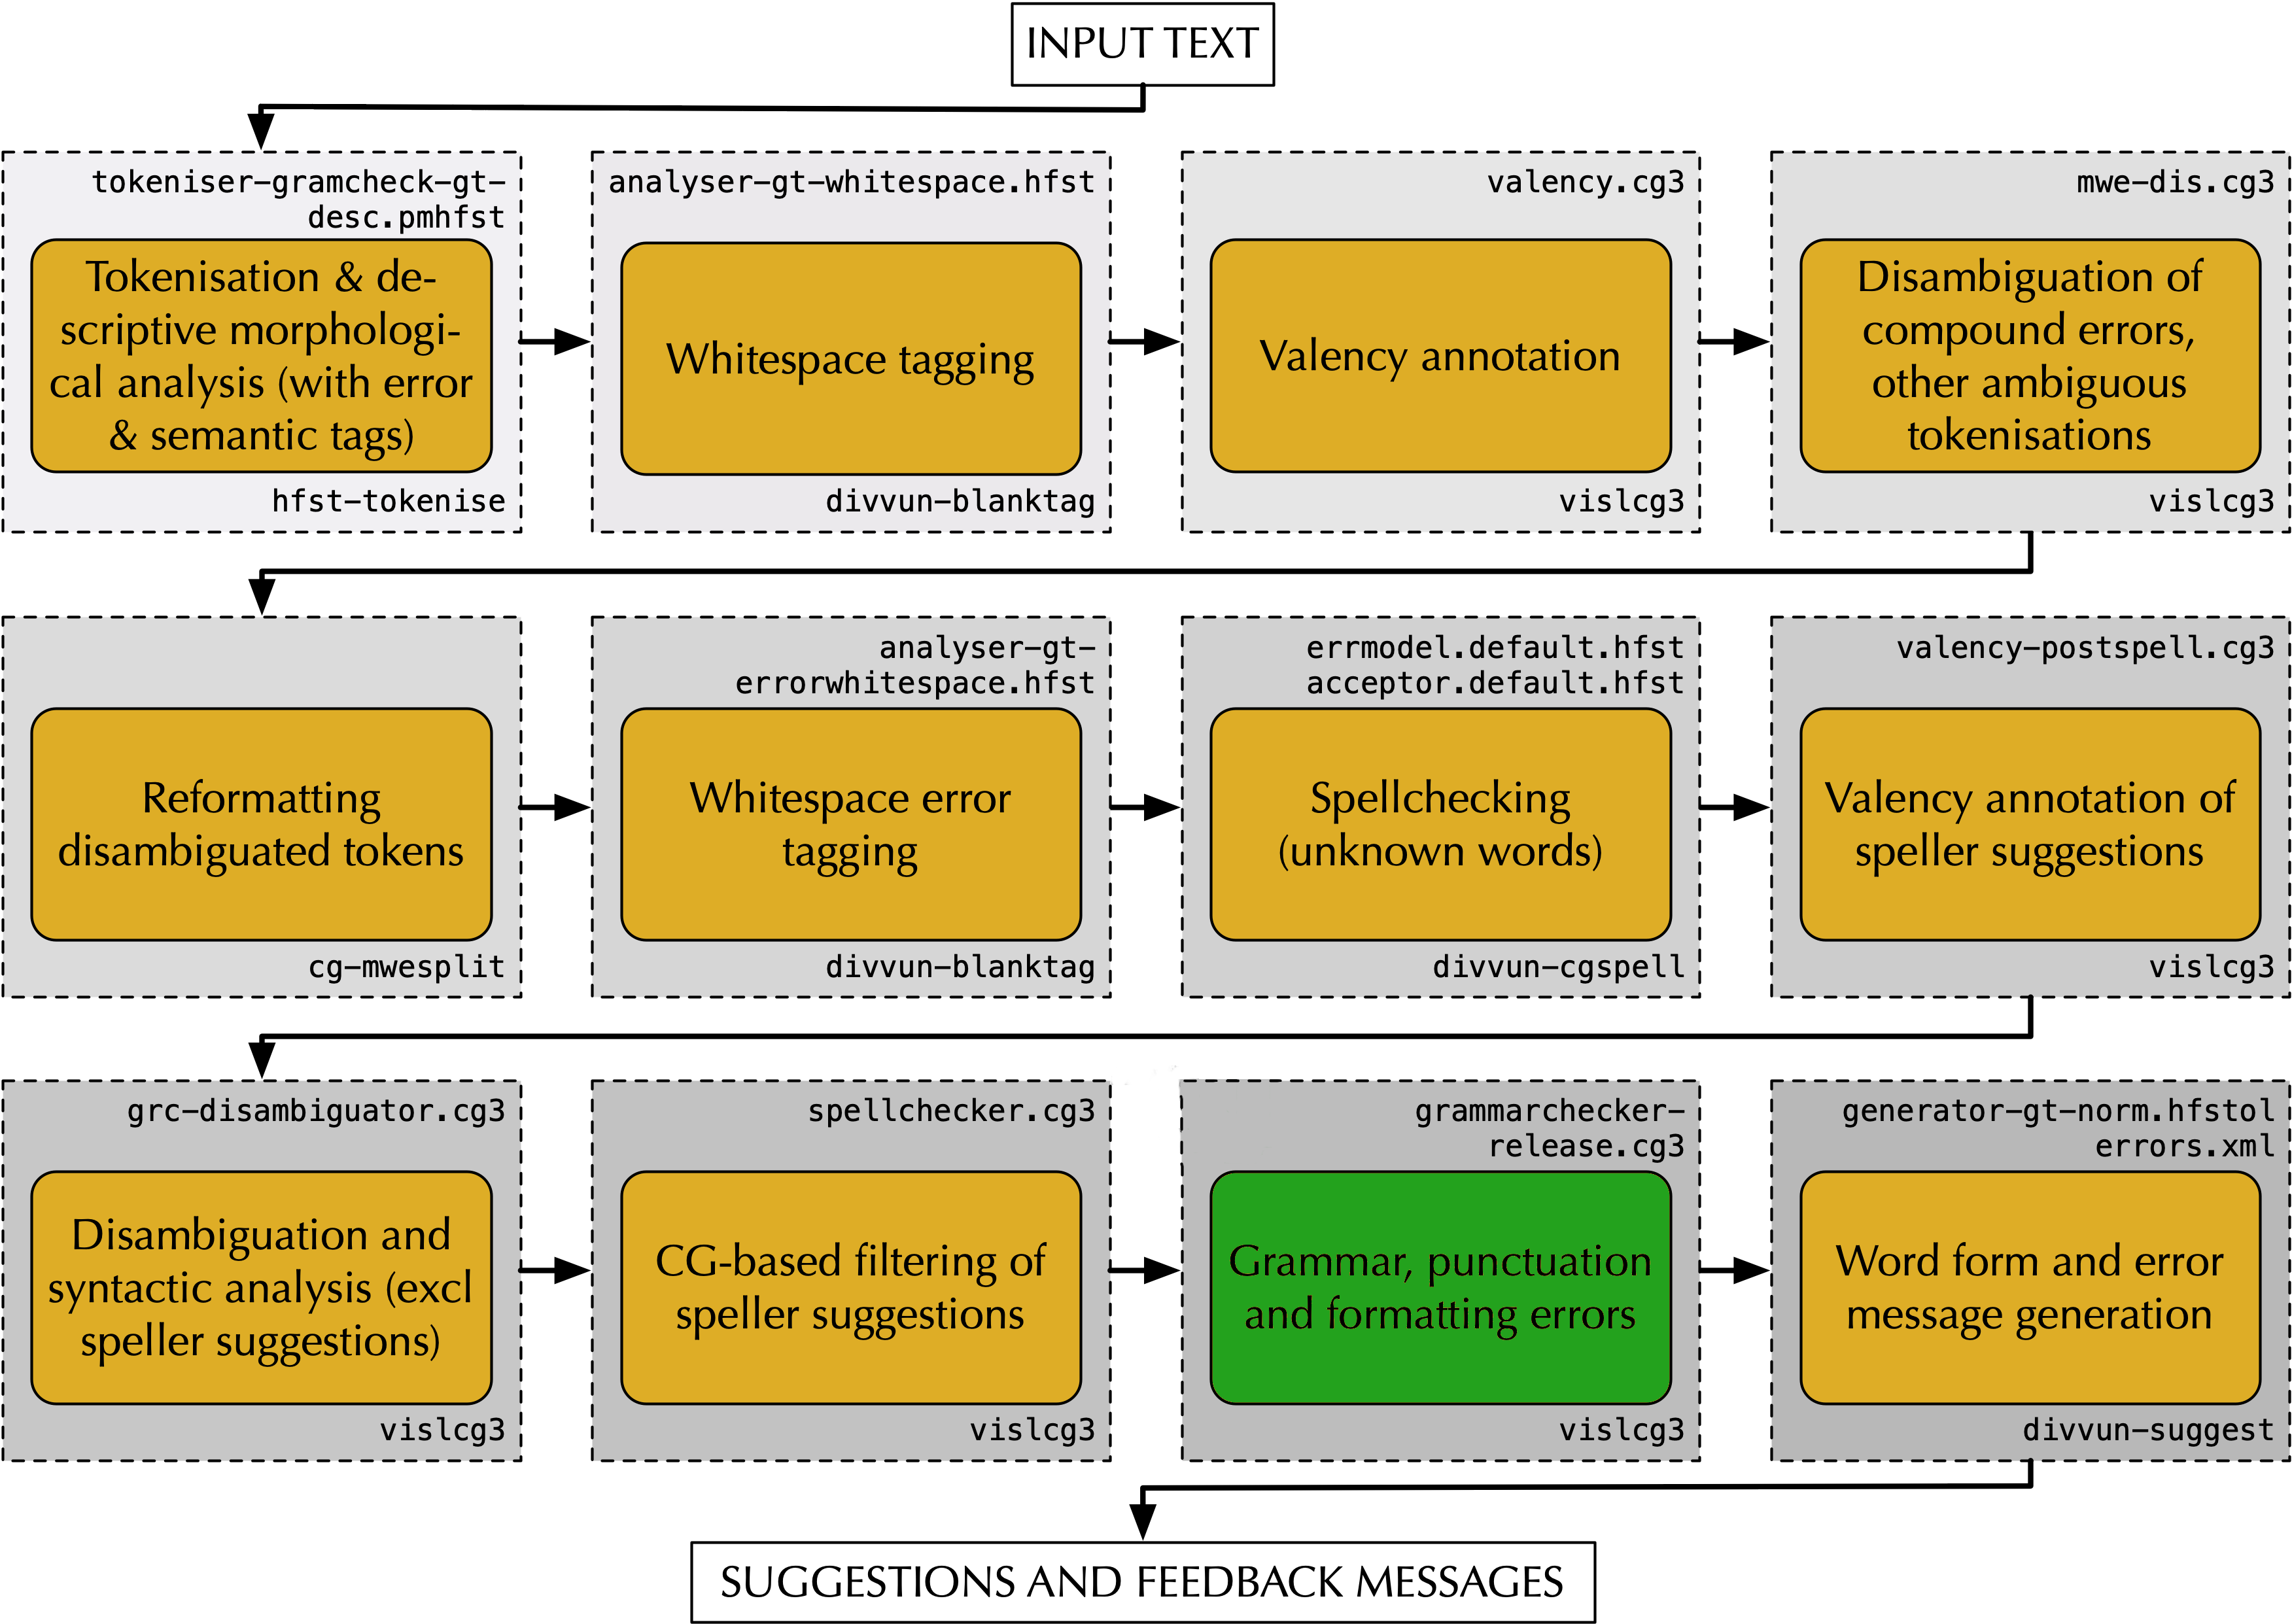
\includegraphics[width=.4\textwidth ]{GramCheckFlow2.0.png}
    \caption{Modular structure of the grammar checkers\label{fig:gramcheckflow}}
\end{figure}

All text data in this work is taken from Sámi international corpus
SIKOR~\cite{sikor_06.11.2018}.  It contains texts in Sámi languages including
South Sámi.

\section{A treebank for South Sámi}


Our VISL CG 3 dependency analyzer for South
Sámi~\cite{wiechetek-kappfjell-2023-south} maps dependencies between word forms
that have received a morphological analysis and a syntactical label.  Each of
these rules builds a partial tree, and combined with each other ideally a full
tree is created. However, the tool is also able to construct partial trees,
which is useful for atypical sentences, ellipses, headlines, in particular
sentences without finite verbs. This is also relevant for South Sámi as
copula-drop is a typical feature of the language.~\cite{Magga2012} It also means
that the tool can construct partial trees for sentences that contain spelling
and grammatical errors or ommitted words.

We ran the dependency parsing tool on 481 sentences and 7,266-token sample
corpus to see how many complete trees it is able to construct.  188 of 481
sentences produce complete parse trees.

One of these complete trees is displayed in Figure~\ref{ngoarpam} showing the
dependency structure of ex.~\ref{daarpesjibie}. It includes a finite verb and
three coordinated infinitives.  The vislcg3 output of the dependency analysis is
displayed as graphical trees for the purpose of visualization. The original
output can be seen in Figure~\ref{ngoarpamvislcg3}, where dependency structures
are expressed by absolute numbers after the hashtag for the position of each
word pointing to the number of the word they are dependent on. In the case of
the finite verb \textit{daarpesjibie} its position in the sentence is \textit{2}
and it points to the root \textit{0} (\#2-$>$0) It creates a full tree despite
the orthographical error in \textit{jih} (should be: \textit{jïh}) as this the
morphological analyzer accounts for some of the typical orthographical errors.
The object \textit{Dam} should be analyzed as dependent on the infinitive
\textit{guarkedh} `understand' instead of \textit{daarpesjibie} `need'.


\exg. Dam daarpesjibie guktie guarkedh, ussjedidh \textcolor{red}{jih} goerehtalledh.\label{daarpesjibie}\\
that\textsc{.acc.sg} need\textsc{.prs.1.pl} for  understand, think and investigate\\
`We need that to understand, think and investigate'.



\begin{figure}
\centering
    \includegraphics[width=1.1\linewidth]{tree2.pdf}
    \caption{Dependency tree for ex.~\ref{daarpesjibie}\label{ngoarpam}}
\end{figure}


\begin{figure}
\scriptsize
   \begin{verbatim}
"<Dam>"
    "dïhte" Pron Pers Sg3 Acc <W:0.0> @OBJ> #1->2
"<daarpesjibie>"
    "daarpesjidh" <mv> V TV Ind Prs Pl1 <W:0.0> @FMV #2->0
"<guktie>"
    "guktie" CS <W:0.0> @CVP #3->4
"<guarkedh>"
    "guarkedh" <mv> V TV Inf <W:0.0> @FS-IMV #4->2
"<,>"
    "," CLB <W:0.0> #5->3
"<ussjedidh>"
    "ussjedidh" <mv> V TV Inf <W:0.0> @IMV #6->4
"<jih>"
    "jïh" CC <W:0.0> @CNP #7->6
"<goerehtalledh>"
    "goerehtalledh" <mv> V TV Inf <W:0.0> @IMV #8->6
"<.>"
    "." CLB <W:0.0> #9->2\end{verbatim}
   \caption{VISL CG3 dependency output\label{ngoarpamvislcg3}}
\end{figure}

The dependency tree for ex.~\ref{maadtoe} is also complete. However, the
dependency structure in Figure~\ref{fig:cfvghbjnk} shows several errors. The
adjective \textit{veaksehke} and the demonstrative pronoun \textit{gaajhkh}
should be dependent on the noun \textit{gielen} instead of the finite verb
\textit{leah}.

The reason for the partial errors in the dependency structure is one grammatical
error in the adjective form \textit{veaksehke} (correct: \textit{veaksehks})
makes it appear a subject in nominative singular instead of an attribute to
\textit{gielen}. \textit{Gaajhkh} can therefore not be identified as adverb
dependent on the adjective. The morphological analyzer is robust enough to
compensate for several spelling errors as the long `i' in three words and
misspelled \textit{aepien} (correct: \textit{aerpien}). They still receive a
morphological and syntactical analysis.


\begin{figure*}
    \centering
    \includegraphics[width=0.7\linewidth]{tree3.pdf}
    \caption{Dependency tree of ex.~\ref{maadtoe}\label{fig:cfvghbjnk}}
\end{figure*}

\ex.
\ag. *\textcolor{red}{Giele} lea mijjen maadtoe, gaajh
\textcolor{red}{veaksehke} \textcolor{red}{gielen} \textcolor{red}{jih} aepien
gaskemsh leah.\label{maadtoe}\\
language be\textsc{.prs.3.sg} our foundation, incredibly strong\textsc{.nom.sg}
language\textsc{.gen.sg} and heritage\textsc{.gen.sg} between
be\textsc{.prs.3.sg}\\
`Language is our foundation, there is an incredibly strong connection between
language and heritage'.
\b. \textcolor{blue}{Gïele} lea mijjen maadtoe, gaajh
\textcolor{blue}{veaksehks} \textcolor{blue}{gïelen} \textcolor{blue}{jïh}
\textcolor{blue}{aerpien} gaskemsh leah.\\


Spelling errors and grammtical non-standard forms are overdimensionally
represented in South Sámi written texts. For most majority languages, spelling
errors and non-standard forms are filtered out by some kind of proofreading. In
addition, writers of majority languages have typically undergone a lot of
training and their writing has undergone a lot of proofreading in their
respective languages school systems.  Figure~\ref{fig:tree1} of a complex
sentence including coordinated demonstrative phrases with a relative clause
displays a number of these typical errors in South Sámi.  Ex.~\ref{vaarjele}
shows all errors with their correction in ex.~\ref{vaarjele2}.

\begin{figure*}
    \centering
    \includegraphics[width=0.549\pagewidth]{tree1.pdf}
    \caption{Dependency analysis for ex.~\ref{vaarjele}\label{fig:tree1}}
\end{figure*}

\ex.
\ag. Gærjagåetie tjööngkie jïh vaarjele gaajhkide tjoejide,
\textcolor{red}{guvvieh} jïh trygkesovveme \textcolor{red}{aamhtesh}
\textcolor{red}{mah} Sveerje \textcolor{red}{olkese}
\textcolor{red}{vadta}.\label{vaarjele}\\
library collect\textsc{.prs.3.sg} and take.care\textsc{.prs.3.sg}
all\textsc{.acc.pl} sound\textsc{.nom.pl}, picture\textsc{.nom.pl} and printed
item\textsc{.nom.pl} which\textsc{.nom.pl} Sweden out give\textsc{.prs.sg.3}\\
`The library collects and takes care of all sound, images and printed items
which Sweden has published'
\b. Gærjagåetie tjööngkie jïh vaarjele gaajhkide tjoejide,
\textcolor{blue}{guvvide} jïh trygkesovveme \textcolor{blue}{aamhtesidie}
\textcolor{blue}{mejtie} Sveerje \textcolor{blue}{bæjhkohte}.\label{vaarjele2}

The coordinated demonstrative phrase does not have consequent case agreement,
the nominative plural nouns \textit{guvvieh} and \textit{aamhtsesh} should be in
accusative case just as their coordinated predecessor \textit{tjoejide}.  The
parsed tree in Figure~\ref{fig:tree1} therefore interprets \textit{guvvieh} as a
new subject to \textit{vaarjele} and does not make it a daughter of
\textit{tjoejide} as it should be. In addition, the nominative plural relative
pronoun \textit{mah} has a case error. It should be accusative \textit{mejtie}
in order to be identified as the object of the finite verb \textit{vadta}.

\section{Creating a preprocessing tool for dependency structure}

In order to create a smoother dependency analysis for South Sámi and facilitate
treebank building, we decided to preprocess the text by means of a hand-written
spelling and grammar checker for the most common error types. We added a
grammatical error annotation layer to SIKOR~\cite{sikor_06.11.2018}. We chose a
182,759-token part of the corpus that had been marked up for spelling errors
already, and classified the grammatical error types on top of those.
Table~\ref{tab:my_label} shows that the corpus contains altogether 740 errors.




\begin{table}[]
    \centering
    \begin{tabular}{cr}
         Morphosntactic errors & 334 \\
         Syntactic errors & 259 \\
         Real-word errors & 147 \\
         Lexical errors & 216 \\
         \midrule
         Non-word spelling & 3,263 \\
    \end{tabular}
    \caption{Error statistics in error annotated text data\label{tab:my_label}}
\end{table}

A demonstrative phrase error as explained in ex.~\ref{vaarjele} is marked as a
unit. The error is then classified with its morpho-syntactic properties---in
this case the nominative plural noun should be in accusative plural---and then
the whole phrase is repeated in its corrected form as below.


\textbf{wrong phrase:}
   \begin{verbatim}
gaajhkide tjoejide, guvvieh
jïh trygkesovveme aamhtesh
   \end{verbatim}
\textbf{error classification:}
   \begin{verbatim}
demphrase,noun,plnom-placc
   \end{verbatim}
\textbf{corrected phrase:}
   \begin{verbatim}
gaajhkide tjoejide, guvvide
jïh trygkesovveme aamhtesidie
   \end{verbatim}

Based on our annotation we decided to write rules for the most frequent error
types that would potentially affect the dependency analysis of the sentences.
Table~\ref{errorrules} shows the selected error types with a few of their
subtypes. The most common errors after adjective form errors and general case
errors (for example in habitive constructions or as a result of valency
violations) are typically agreement errors, both between subject and verb and
noun phrase internal agreement (including quantifiers and demonstratives).

\begin{table*}[]
    \centering
    \begin{tabular}{lll}
    \bf rule type & \bf error & \bf correction \\
    \toprule
        demonstrative phrase case agreement & Dem Nom  &    \\
        \midrule
         numeral phrase agreement & Num N.Nom.Sg. & Num N.Nom.Pl. \\
         numeral phrase agreement & Num N.Pl. & Num N.Sg. \\
            \midrule
         habitive constructions  & Nom.\ copula Nom. & Gen.\ copula Nom. \\
        infinitive after auxiliary & aux vfin & aux Inf \\
        postposition complement & Acc Po & Gen Po \\
        \midrule
        subject verb agreement & 1. Du & 3. Pl. \\
       subject verb agreement & 3. Pl. & 3. Sg. \\
        subject verb agreement & 2. Sg. & 3. Pl. \\
       subject verb agreement & 3. Sg. & 3. Pl. \\
        subject verb agreement & Inf. & 3. Pl. \\
              \midrule

        phrasal verb lex verb & V Adv & V \\
        unidiomatic phrasal verb & V Adv & V Adv \\
        \midrule
        negation past tense agreement & & \\
        negation verb phrase & Neg Inf & Neg Conneg \\
        \midrule
        adjective forms & attr & Nom. Sg. \\
                        & attr & Nom. Pl. \\
                        & Nom. Sg. & attr \\
                        & Nom. Sg. & adv \\
        \bottomrule
    \end{tabular}
    \caption{Rule types checked in the South Sámi grammar checking
    tool\label{errorrules}}
\end{table*}




South Sámi demonstrative phrase and numeral phrases differ from Germanic
structures and follow complex rules, which is why errors are common. In
demonstrative (and indefinite) phrases typically pronouns and nouns agree in
number and case. In numeral phrases, on the other hand, only nominative agrees
in number and case. In all other cases, the noun is in singular after all
numbers above \textit{one}.

In ex.~\ref{gaajhkh}, the indefinite pronoun nominative plural \textit{gaajhkh}
`all' needs to be changed to accusative \textit{gaajhkide} ` to all' because of
the subsequent accusative noun \textit{maanide} `children' and its agreement
requirements.

\ex.
\ag. *Seabradahken dåarjoe maanasåjhtose edtja \textcolor{red}{gaajhkh} maanide
båetedh.\label{gaajhkh}\\
community\textsc{.sg.ine} support childcare\textsc{.sg.ill}
should\textsc{.prs.3.sg} all\textsc{.pl.nom} child\textsc{.pl.ill}
come\textsc{.inf}\\
`Community support for childcare should reach all children'
\b. Seabradahken dåarjoe maanasåjhtose edtja \textcolor{blue}{gaajhkide} maanide
båetedh.

We also need to account for exceptional use of numerals such as in the following
sentence~\ref{nulle-objekt}, where \textit{nulle} `zero' is actually used as
part of a compound `zero-object' and not as a quantifier.

\ex. Voestes aejkien manne \textbf{nulle objeekten} bïjre govlim utnim luste
goerehtidh maam ij våajnoes aktene raajesisnie.\label{nulle-objekt}\\
`The first time I heard about the zero object, I thought it was fun, which
wasn't in a sentence'.

Apart from demonstrative phrase, numeral phrase and nominal phrases involving
adjectives, also postpositional phrases can alter the dependency structure in
parts of the tree. Ex.~\ref{janne} displays a typical case error in dependents
of postpositions. In South Sámi, the correct form is genitive case. However, a
frequent error is to use accusative case as \textit{dam} `the' instead of
genitive \textit{dan}  `the'. These errors can also involve coordinated noun
phrases such as in ex.~\ref{vuejnedh}.

\ex.
\ag. Janne åådtje munnjien \textcolor{red}{dam} bïjre mænngan soptsestidh.\label{janne}\\
Janne get\textsc{.prs.3.sg} I\textsc{.ill} that\textsc{.acc} about later talk\textsc{.inf}\\
Janne can talk to me about it later.\\
\b. Janne åådtje munnjien \textcolor{blue}{dan} bïjre mænngan soptsestidh.\\

\ex.
\ag. Mijjieh sïjhtebe vuejnedh buarastehtemem staaten,
\textcolor{red}{faagesiebrieh jïh barkoevedtijh} gaskem juktie destie
baalhkajoekehts nyjsenæjjide\label{vuejnedh}\\
we want\textsc{.prs.1.pl} see\textsc{.inf} handshaking\textsc{.acc}
state\textsc{.gen.sg}, tradeunion\textsc{.gen.pl} and employer\textsc{.gen.pl}
between\\
`We want to see a handshake between the state, the tradeunion and the employers'.
\b. Mijjieh sïjhtebe buarastehtemem vuejnedh staaten,
\textcolor{blue}{faagesïebri jïh barkoevedtiji} gaskem\\

Other frequent case errors regard habitive constructions such as the one in
ex.~\ref{gaajhkesh}, where the possessor role needs to be in genitive case
(\textit{Gaajhkesi}) instead of nominative case \textit{Gaajhkesh} `everyone'.
Only then can they be correctly identified as part of the habitive structure in
a dependency analysis.

\ex.
\ag. \textcolor{red}{Gaajhkesh} leah reaktah årromesæjjan.\label{gaajhkesh}\\
everyone\textsc{.nom.pl} are\textsc{.prs.3.pl} right\textsc{.nom.pl} housing\textsc{.ill.sg}\\
`Everbody has the right to a place to live'.\\
\b. \textcolor{blue}{Gaajhkesi} leah reaktah årromesæjjan.\\

Verb phrase errors typically regard subject-verb agreement as in
examples~\ref{vuelkebe} and~\ref{edtjebe}, where the verb form needs to be in
first person dual instead of first person plural since two and no more people
are performing the action. In order to match the verb with its subject, it needs
to be in its correct person and number.

\ex.
\ag. Daan biejjien Manne jïh Janne \textcolor{red}{vuelkebe} Afrikese, eejehtæmman\label{vuelkebe}\\
Today I and Janne go\textsc{.prs.1.pl} Africa\textsc{.ill.sg} vacation\textsc{.ill.sg}\\
`Today I and Janne are going to Africa for vacation'.\\
\b. Daan biejjien Manne jïh Janne \textcolor{blue}{vuelkien} Afrikese, eejehtæmman\\


\ex.
\ag. Mænngan Janne jïh manne \textcolor{red}{edtjebe} tjaetsieskuvterem vuejedh!\label{edtjebe}\\
Later Janne and I will\textsc{.prs.1.pl} water.scooter\textsc{.acc.sg}  drive\textsc{.inf}\\
`I and Janne will later drive a water scooter'.\\
\b. Mænngan Janne jïh manne \textcolor{blue}{edtjien} tjaetsieskuvterem vuejedh!\\

The following constraint grammar rules in Figure~\ref{smademphrase} add
errortags to (multiple) demonstrative/indefinite pronouns noun combinations and
relate them to each other (ADDRELATION) to create a unified error that will be
visualized as one error.

\vspace{5pt}
\begin{figure}
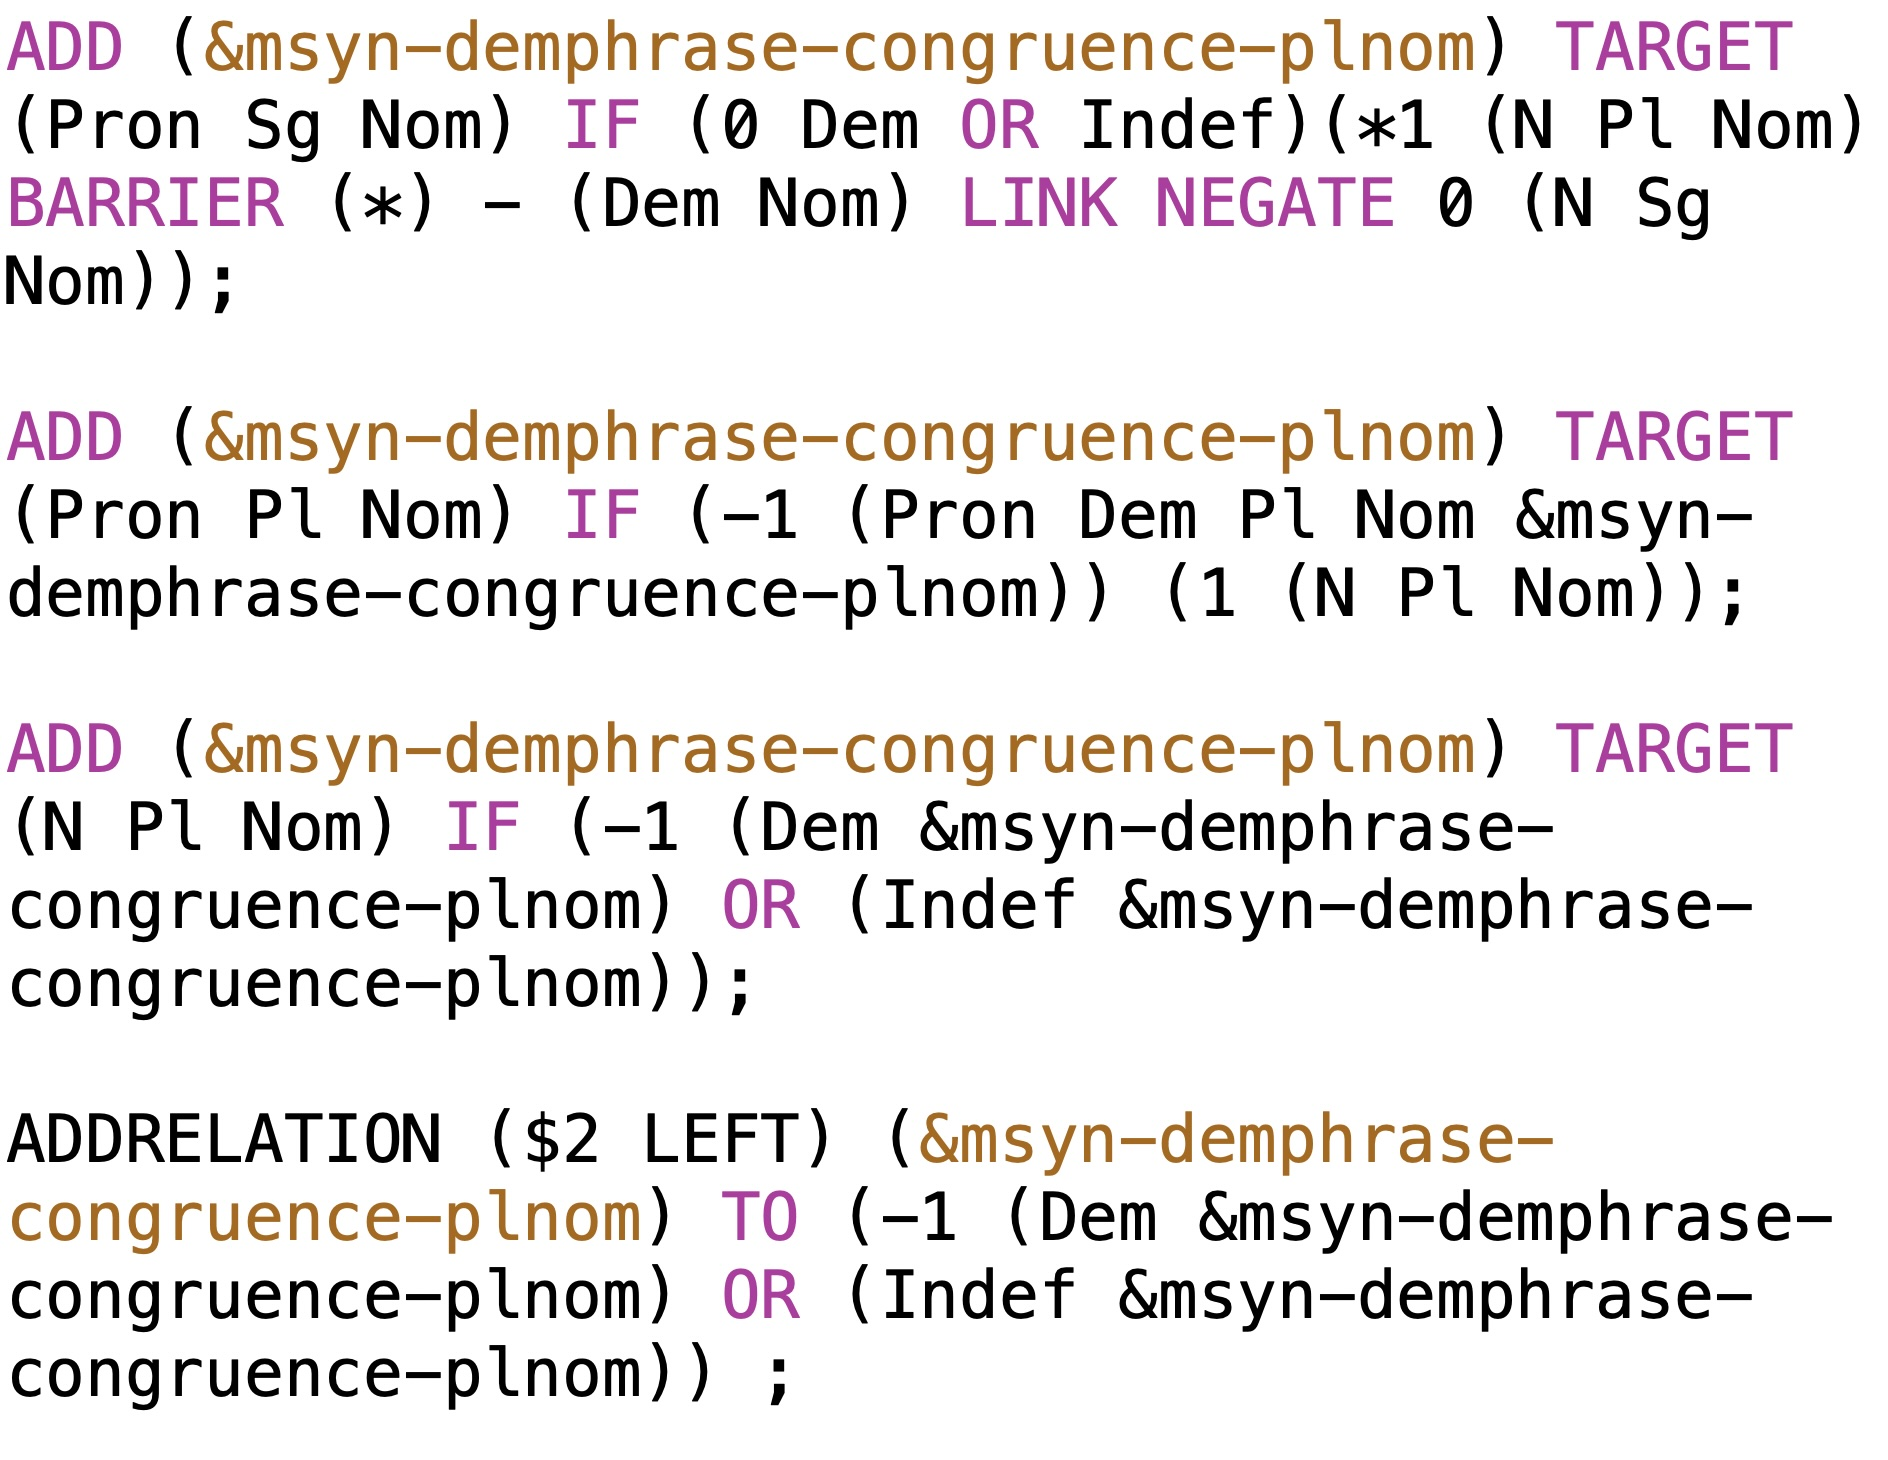
\includegraphics[scale=0.2]{smademphrase.jpg}
\caption{Constraint grammar rules adding error tags to demonstrative phrases\label{smademphrase}}
\end{figure}
\vspace{5pt}

\begin{table}[]
    \centering
    \begin{tabular}{lrrr}
         Dataset &  Full trees & Partial \\
         \midrule
         Originals & 915 & 1296 \\
         GEC &  1390 & 811 \\
         Hand-corrected & 1259 & 948 \\
    \end{tabular}
    \caption{Automatically parsed dependency trees in SIKOR\label{tab:my_label}}
\end{table}

\section{Evaluation}

We chose a 100 sentence test corpus, part of SIKOR, to manually evaluate the
post spell- and grammar checking dependency analysis and got the following
results.  73 of 100 sentences received a correct dependency analysis (73\%).

\begin{figure}
    \centering
    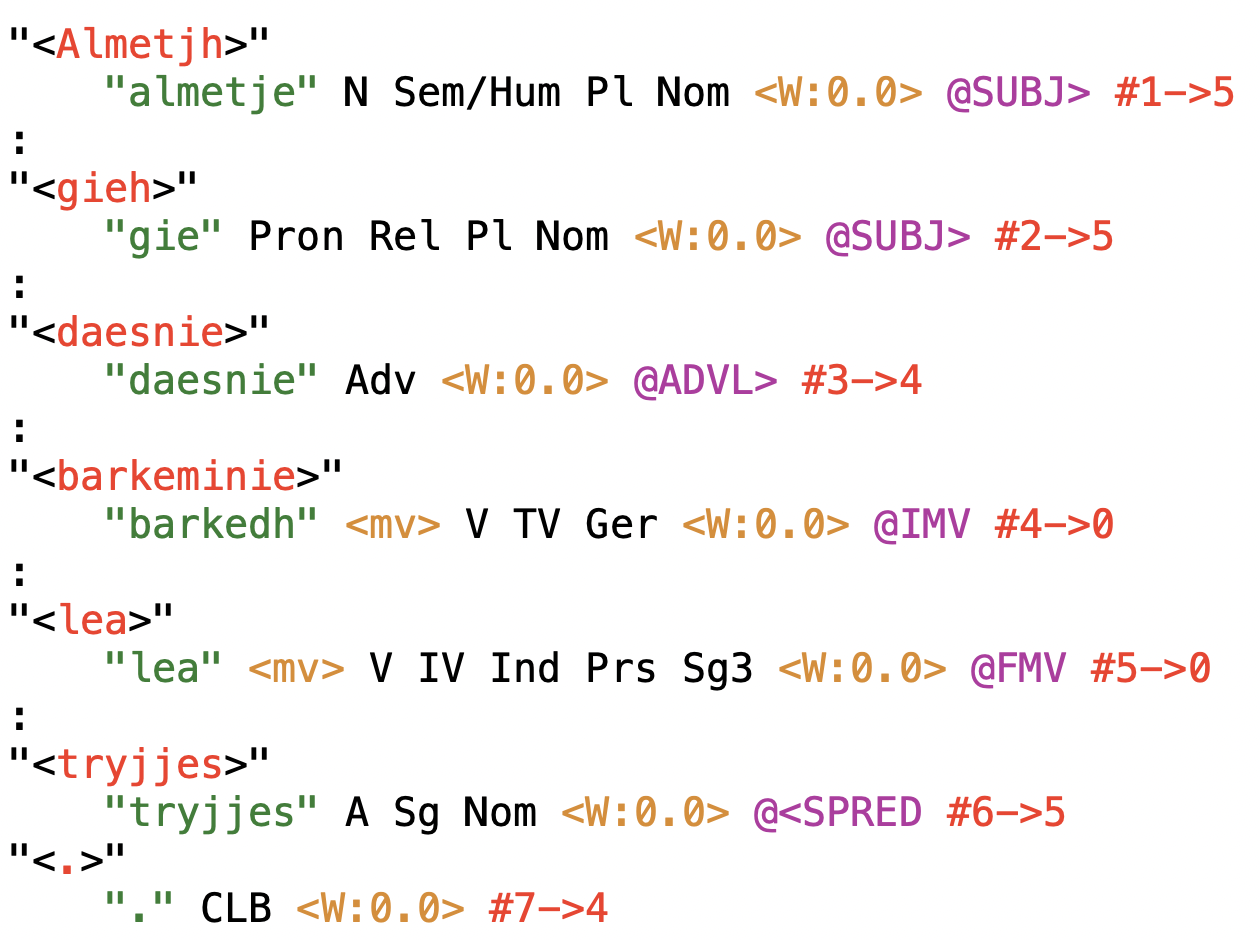
\includegraphics[width=.5\textwidth ]{copdropsma.png}
    \caption{Copula drop dependency analysis of
    ex.~\ref{almetjh}\label{copdrop}}
\end{figure}


\exg. Almetjh gieh daesnie barkeminie, lea tryjjes.\label{almetjh}\\
people\textsc{.nom.pl} who\textsc{.nom.pl} here working\textsc{.ger}
be\textsc{.prs.1.sg} friendly\textsc{.nom.sg}\\
`People who are working here are friendly'.

Copula drop is a known issue in South Sámi describe thoroughly
in~\cite{ylikoski2022}, and it appears in different forms---the sentence can
drop the auxiliary in periphrastic verbal constructions as the one in the
previous example, leaving only the non-finite verb form (past participle, gerund
etc.).  It can also be dropped in copula constructions, leaving only the subject
and the predicate. When there are complex sentences with main- and subclause,
where the mainclause has copula drop, while the subclause has a finite verb
form, the automatic analyzer often analyses the finite verb form of the
subclause as the daughter of the root, instead of making it the daughter of the
non-finite verbform of the main clause. South Sámi syntax poses challenges to
machine-based dependency analysis, which languages with required finite verbs do
not, and new solutions need to be carefully investigated.

Other reasons for failing dependencies are remaining spelling and grammar errors
(6), and shortcomings in the analysis regarding coordination (7) and finding the
correct verbal mother (12).
\section{Conclusion}

Low resource languages like South Sámi need language resources and treebanks
like all other languages. Our approach has taken into account that South Sámi
lacks human resources to mark up large amounts of texts to create a treebank by
applying a rule-based tool to do so. Instead, we have used our human resources
to create and improve rule-based grammar checking and dependency tools so that
we can post-edit our treebank with much less effort than creating it from
scratch. We have further identified one of the causes of noise in the creation
of such resources---spelling and grammatical errors. We therefore enhanced a
marked-up error corpus to systematically identify the most frequent grammatical
errors that can get into the way of automatic dependency annotation. These
include both, errors on the noun phrase and the verb phrase
level---demonstrative phrases, numeral phrases, adjectival forms, case errors in
habitive constructions and postpositional phrase being a few of them. Based on
this analysis we have written rules for all the previous error types to
automatically identify and correct these errors and preprocess the input text
for the dependency analyzer.  We can see that the number of full and partial
trees increases with the correction of these grammatical errors, and our current
dependency tool gives us 91.3\%.  As a next step, we plan to improve our
dependency tool and with some human post-editing create the first South Sámi
treebank.

We have seen that our method is an efficient way of creating a treebank, a
dependency tool and a grammar checker at that same time, all of which can be
used as language resources and proofing tools by the South Sámi language
community.




\bibliography{syntaxfest2025}
\bibliographystyle{unsrt}

\appendix


\end{document}
